\documentclass[]{article}
\usepackage[margin=2cm]{geometry}
\usepackage{graphicx}

\begin{document}

\begin{center}
\textsc{\Huge Curvas de Rotacion de una Galaxia}\\[0.8cm]
\Large Juan Prada M \\[0.5cm]
\Large 201425533 \\[0.5cm]
\end{center}

\newcounter{mysection}
{Datos Experimentales y Modelo}\\[0.1cm]

\begin{figure}[!ht]
{
    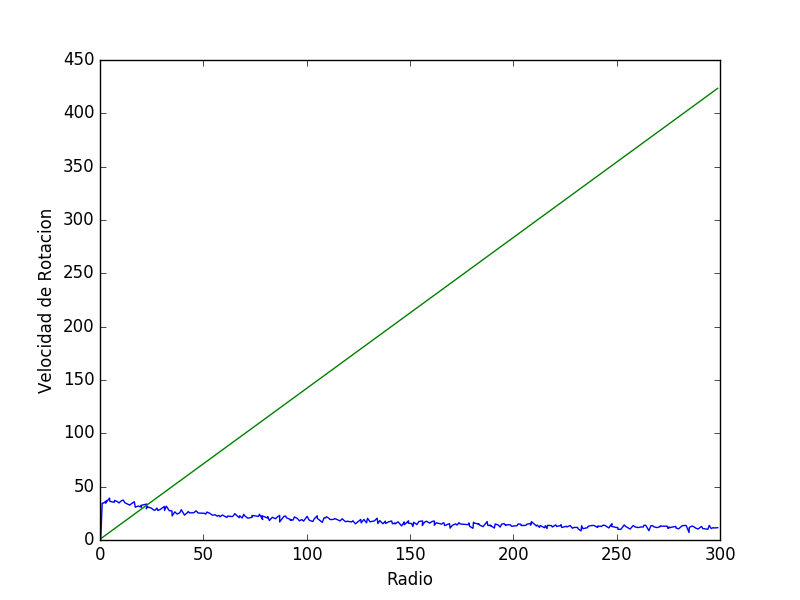
\includegraphics[width=\linewidth]{DatosyModelo.png}
    \caption{Datos y Modelo}
}
\end{figure}

\end{document}
